\section{Aufbau des Clients}

Aus den oben genannten Anforderungen kann eine grobe Architektur abgeleitet werden:

%Hier ein erstes Klassendiagramm zu  
%     * BaseClient
%     * Client 
%     * Connection 
%     * Listener
%     * NotifyData
%bzw. deren Verbindung

\subsection{Hauptklassen}

\begin{figure}[htb!]
	\centering
        \includegraphics[scale=0.55]{BaseClientCollab.png}
	\caption{Kollaborationsdiagramm zu BaseClient}
	\label{collab_base_client}
\end{figure}

\subsubsection{BaseClient}
Diese Klasse bildet die Basis zur eigentlichen Clientklasse. Sie kann nicht direkt instanziert werden,
und verwaltet administrative Tätigkeiten wie den eigentlichen Verbindungsaufbau \ref{seq_client_connect} an sich. 
Desweiteren bietet er einfache Funktionen zum eintreten und verlassen des ,,Idlemodes'' an.
\\
Geht die verbindung verloren (ohne dass \emph{disconnect()} explizit aufgerufen wurde), so versucht sich der BaseClient periodisch sich zu reconnecten.
Das Intervall in dem diese Versuche geschehen soll von ,,settings.connection.reconnectinterval'' gelesen werden.
\\
Er soll mindestens folgende public Methoden bieten:

Gibt eine Referenz auf das zugrunde liegende MPD::Connection Objekt zurück. 
AbstractClientExtension benötigt dies.
\begin{verbatim}
        Connection& get_connection(void);
\end{verbatim}

Prüft ob eine Verbindung besteht.
\begin{verbatim}
        bool is_connected(void);
\end{verbatim}
Die get\_status() Funktion soll den letzten aktuellen MPD::Status zurückliefern,
oder NULL falls nicht verbunden. 
\begin{verbatim}        
        Status * get_status(void);
\end{verbatim}

Die folgenden Funktion rufen einfach die entsprechenden Funktionen von MPD::Listener auf,
prüfen aber zusätzlich noch ob eine Verbindung besteht:
\begin{verbatim}
        EventNotifier& signal_client_update(void);
        ConnectionNotifier& signal_connection_change(void);

        void force_update(void);
        void go_idle(void);
        void go_busy(void);
\end{verbatim}

\subsubsection{Listener}
Der Listener verwaltet alles was mit dem Betreten und Verlassen des ,,Idlemodes''
zutun hat. Er setzt den eingangs beschriebenen Watchdog auf die asynchrone Verbindung an,
und parst die entsprechenden Antworten des Servers von Hand. 
\\
Er verfügt zudem über ein ,,EventNotifer'' (ein sigc::signal)
Periphere Klasse können sich so über connect() registrieren.
Bemerkt der Listener Events so ruft er emit() auf dem sigc::signal auf
und teilt allen anderen Modulen so mit welche events geschehen sind.
\\
Es folgt eine Liste von Funktionen die der Listener mindestens haben soll.
\\
enter() tritt in den ,,Idlemode'' ein. Es ist ab diesem Punkt nicht mehr erlaubt Kommandoes zu senden.
leave() ist das genaue Gegenteil von enter() und verlässt den ,,Idlemode'' sodass Kommandoes gesendet werden können.  
is\_idling() sollte selbsterklärend sein.
\begin{verbatim}
       bool enter(void);
       void leave(void);
       bool is_idling(void);
\end{verbatim}

Es soll zudem eine force\_update() Funktion geben die ,,künstlich'' alle Events auslöst.
Dies ist nützlich bei der Initialisierung.
\begin{verbatim}
       void force_update(void);
\end{verbatim}

\subsubsection{Connection}
\begin{figure}[htb!]
	\centering
        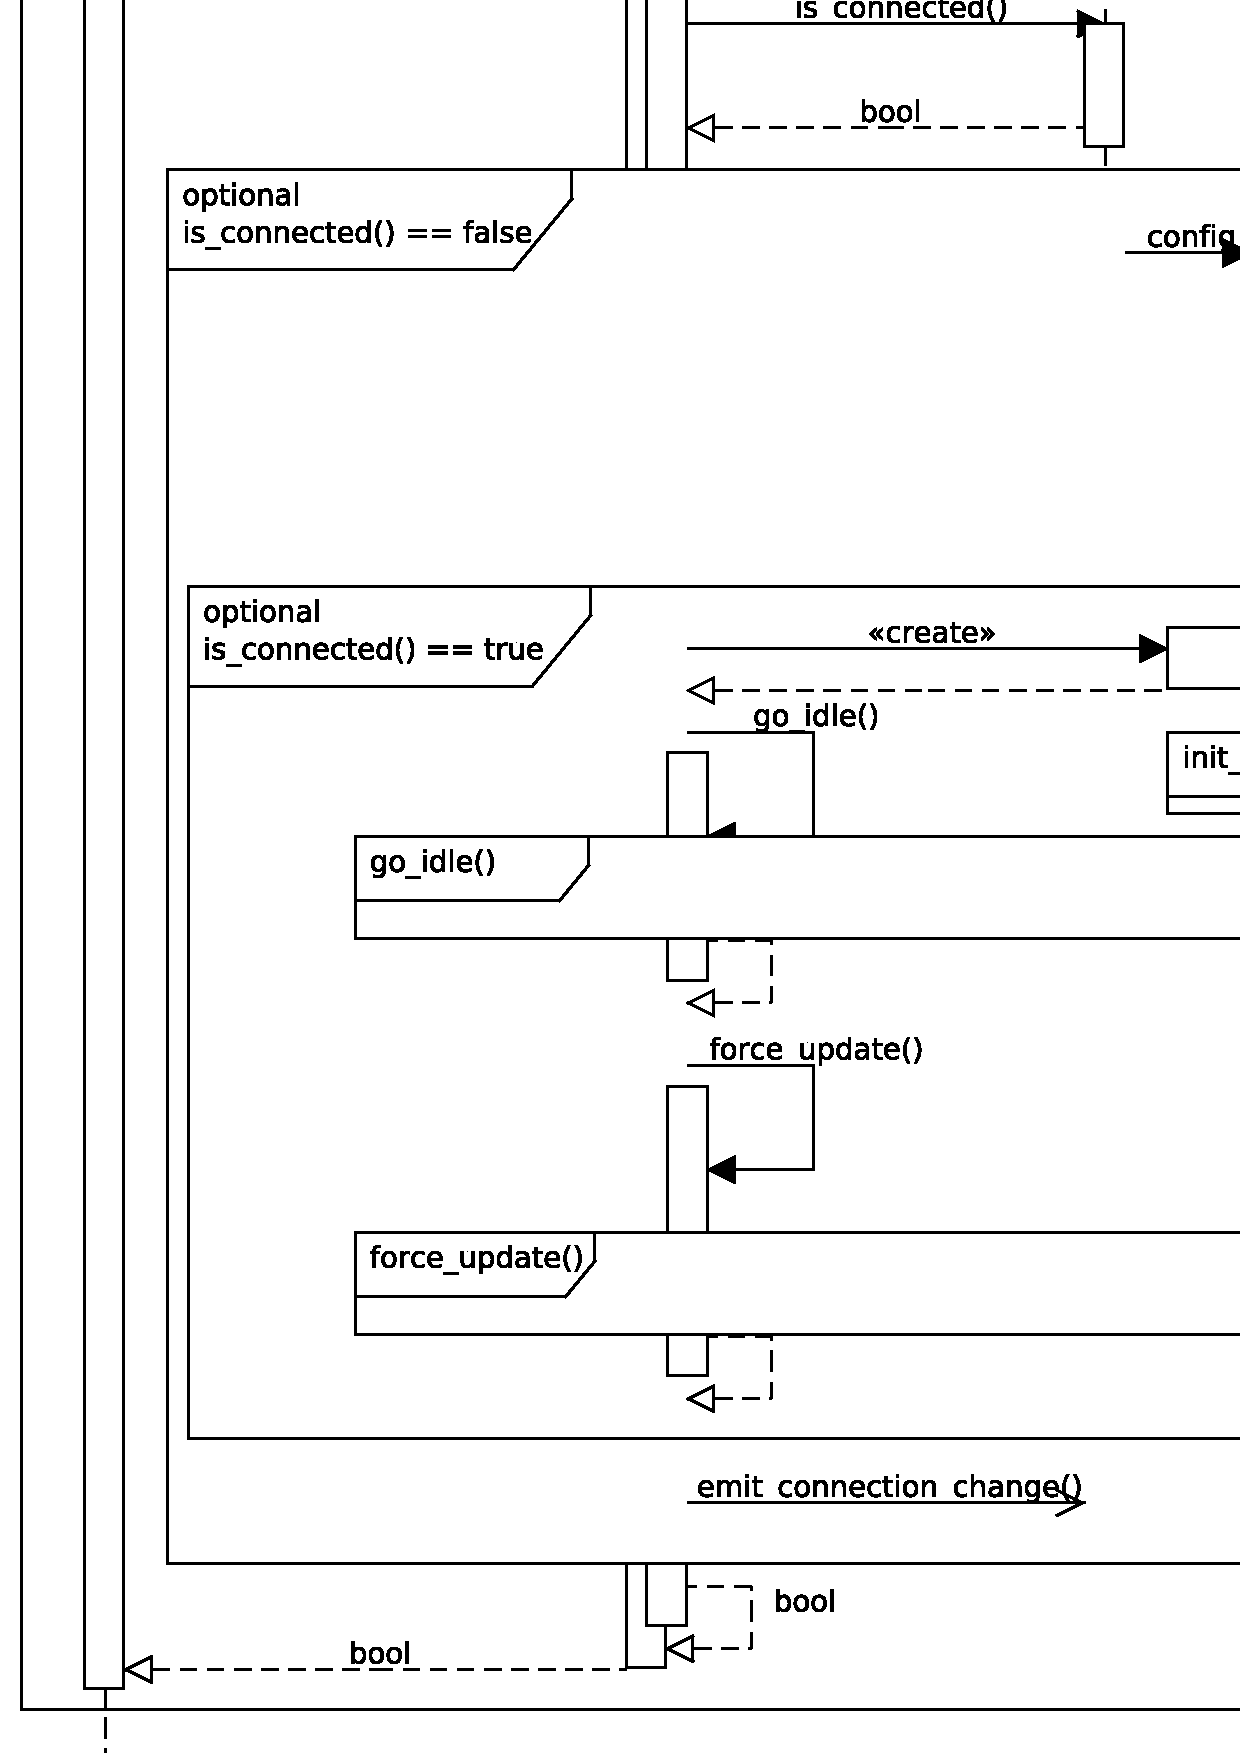
\includegraphics[scale=0.5]{ConnectSequence.pdf}
	\caption{Sequenzdiagramm zum Verbindungsaufbau}
	\label{seq_client_connect}
\end{figure}
Diese Klasse stellt eine Art Wrapper um die mpd\_connection Struktur von libmpdclient da.
Neben den eigentlichen connect() und disconnect() Methoden.
Sie hält zudem den letzten Host als Membervariable um feststellen zu können ob sich dieser zwischen 
zwei Verbindungsvorgängen geändert hat. Desweiteren bietet sie eine Schnittstelle um sich über Fehler informieren zu lassen (signal\_error())
\\
Es folgt eine Liste von Funktionen die mindestens vorhanden sein sollten.
Ein boolean-Rückgabewert von true zeigt stets Erfolg an.
\\
connect() soll die eigentliche Verbindung herstellen, disconnect() löscht die Verbindung wieder.
get\_connection() liefert einen Pointer auf die darunter liegende C-Struktur. Alle 4 Funktionen prüfen 
zudem intern bereits auf Fehler.
\begin{verbatim}
    bool is_connected(void);
    bool connect(void);
    bool disconnect(void);
\end{verbatim}

Zur Implementierung konkreter Kommandoes wird die darunterliegende C-Struktur benötigt.
\begin{verbatim}
    mpd_connection * get_connection(void);
\end{verbatim}

Auf den Rückgabewert dieser Funktionen kann sigc::signal::connect() aufgerufen werden, 
um einen Funktionspointer zu registrieren der aufgerufen wird sobald ein Fehler eintritt,
bzw. sich die Verbindung ändert. Die Prototypen sollen jeweils sein:
\begin{verbatim}
    typedef sigc::signal<void, bool,mpd_error> ErrorNotify;
    typedef sigc::signal<void,bool,bool> ConnectionNotifier;
    
    ErrorNotify& signal_error(void);
    ConnectionNotifier& signal_connection_change(void)
\end{verbatim}

Die Prototypen entsprechen den Templateargumenten in den typedefs:
\begin{verbatim}
    void error_handler(bool is_fatal, mpd_error err_code);
    void conn_change_handler(bool server_changed, bool is_connected); 
\end{verbatim} 

libmpdclient verbietet es weitere Kommandos an den Server zu senden wenn vorher ein Fehler passiert ist.
Fehler müssen zuerst mit \emph{mpd\_connection\_clear\_error()} ,,bereinigt'' werden. 
Dies tut check\_error(). Die Funktion wird normal nicht selbst aufgerufen, da sie von allen anderen Funktionen der Klasse
implizit aufgerufen wird. Ist ein Fehler passiert so werden alle Klienten die sich zuvor
mit signal\_error() registriert haben benachrichtigt. 
\begin{verbatim}
    bool check_error(void);
\end{verbatim}


\subsubsection{Client}
\begin{itemize}
    \item Der Client erbt von BaseClient und implementiert konkrete Commandos wie ,,play'',,,random'' etc.
    \item Er bietet zudem Schnittstellen zur Befüllung der Datenbank, der Queue und des Playlistmanagers
    \item Er bietet die Methoden connect() und disconnect() 
    \item Ist in der config ,,settings.connection.autoconnect'' gesetzt so connected er sich automatisch.
    \item Er bietet zudem eine schnittstelle um sich beim listener zu registrieren und im falle von 
        änderungen des connection zustands benachrichtigt zu werden.
\end{itemize}

connect() und disconnect() stellen die öffentliche Schnittstelle zum Verbinden dar.
Sie rufen intern lediglich \_\_connect() bzw. \_\_disconnect() von MPD::BaseClient auf.
\begin{verbatim}
    void connect(void);
    void disconnect(void);
\end{verbatim}

Die ersten 4 Funktionen sollten offensichtlich sein.
playback\_crossfade() weist den MPD Server an zwischen 2 Songs weich zu überblenden. Die Überblendzeit wird
dabei in Sekunden übergeben, wobei 0 das Crossfade komplett ausschaltet.
playback\_pause() hält die aktuelle Wiedergabe an, oder setzt sie fort wenn bereits angehalten.
playback\_seek() springt in den Song mit der ID song\_id an die Stelle abs\_time in Sekunden.
Die ID des momentan spielenden Songs kann durch get\_status() gefunden werden.
Alle Funktionen (mit Ausnahme von playback\_crossfade) im nächsten Block lösen ein "player" Event aus.
\begin{verbatim}
    void playback_next(void);
    void playback_prev(void);
    void playback_stop(void);
    void playback_play(void);
    void playback_crossfade(unsigned seconds);    
    void playback_pause(void);
    void playback_seek(unsigned song_id, unsigned abs_time);
\end{verbatim}

4 Funktionen um jeweils \it random, consume, repeat\rm und \textit{single}-modi umzuschalten.
\begin{verbatim}
    void toggle_random(void);
    void toggle_consume(void);
    void toggle_repeat(void);
    void toggle_single(void);
\end{verbatim}

Todo...
\begin{verbatim}
    void play_song_at_id(unsigned song_id);
    void playlist_save(const char * name);
\end{verbatim}   

Funktionen zum Bearbeiten der Queue. 
\begin{verbatim}
    void queue_add(const char * url);
    void queue_clear(void);
    void queue_delete(unsigned pos);
\end{verbatim}

database\_update() sendet MPD Server Hinweis um DB zu aktualisieren.
database\_rescan() sendet MPD Server Hinweis um DB neu einzulesen (teuer).
\begin{verbatim}
    void database_update(const char * path);
    void database_rescan(const char * path);
\end{verbatim}

Setzen des volumes von 0-100; Abfrage des Volumes sollte über get\_status() erfolgen.
\begin{verbatim}
    void set_volume(unsigned vol);
\end{verbatim}

Folgende Funktionen sollen von AbstractItemGenerator voll implementiert werden.    
\begin{verbatim}

    void fill_queue(AbstractItemlist& data_model);
    void fill_queue_changes(AbstractItemlist& data_model,
                            unsigned last_version,
                            unsigned& first_pos);
    void fill_playlists(AbstractItemlist& data_model);
    void fill_outputs(AbstractItemlist& data_model);
    void fill_filelist(AbstractItemlist& data_model, const char * path);
\end{verbatim}

\subsubsection{NotifyData}
\begin{itemize}
    \item Speichert den Status, den aktuellen Song und die aktuelle Datenbankstatistik
    \item Der Listener...
        \begin{itemize}
            \item instanziert NotifyData im Konstruktor
            \item sagt NotifyData wann er sich updaten soll (update\_all())
            \item gibt bei einem Event eine Referenz auf NotifyData an alle registrierten Module weiter,
                damit diese konkrete Informationen beziehen können.
        \end{itemize}
\end{itemize}

\begin{verbatim}
        Status& get_status(void);
        Statistics& get_statistics(void);
        Song * get_song(void);
        Song * get_next_song(void);
\end{verbatim}

Test
\begin{verbatim}
        /**
         * @brief Update internal client state
         */
        void update_all(unsigned event = UINT_MAX);
\end{verbatim}


\subsection{Weitere Klassen}
Desweiteren gibt es einige weitere Klassen die am Rande eine Rolle spielen,
und meist Objektorientierte Wrapperklassen für die C-Strukturen von libmpdclient bereitstellen.

\subsubsection{Song}

Die Song Klasse für Wrapper für mpd\_song Struktur und die dazugehörigen Klassen (libmpdclient).
Soll alle Funktionen von libmpdclient \footnote{http://www.musicpd.org/doc/libmpdclient/song\_8h.html} anbieten,
diese werden hier nur aufgelistet aber nicht erklärt da sie genau wie ihre Vorbilder funktionieren:

\begin{verbatim}
    const char * get_path(void);
    const char * get_tag(enum mpd_tag_type type, unsigned idx);
    unsigned get_duration(void);
    time_t get_last_modified(void);
    void set_pos(unsigned pos);
    unsigned get_pos(void);
    unsigned get_id(void);
\end{verbatim}

MPD::Song soll zudem eine Funktion bieten um die Metadaten des Songs in einer printf änhlichen Art als String zurückzuliefern:
\begin{verbatim}
    Glib::ustring song_format(const char* format, bool markup=true);
\end{verbatim}

Ein beispielhafter Aufruf:
\begin{verbatim}
    SomeSong.song_format("Artist is by ${artist}") 
\end{verbatim}

Die folgenden Tagarten sollen dabei unterstützt werden (sie spiegeln in etwa die mpd\_tag\_type Enumeration von libmpdclient wieder)
Foldende Tags sollen daher unterstützt werden: \it artist, title, album, track, name, data, album\_artist, genre, composer, performer, comment, disc\rm.
Ist ein Escapestring nicht bekannt, so wird er nicht escaped. Ist der tag nicht vorhanden soll mit "unknown" escaped werden.


\subsubsection{Directory}
Die Directory Klasse ist Wrapper für mpd\_directory C-Strukutr. Diese wird als Anzeige für ein Verzeichniss benutzt,
jedoch nicht als Container für andere Elemente.

Entsprechend implementiert bietet MPD::Directory nur:
\begin{verbatim}
    void get_path(void);
\end{verbatim}

Dies ist von der AbstractComposite vorgegeben.

\newpage
\subsubsection{Statistics}
Die Statistics Klasse ist Wrapper für mpd\_stats, implementiert gemäß \url{\\http://www.musicpd.org/doc/libmpdclient/stats\_8h.html}
folgende Funktionen:
\begin{verbatim}
    unsigned get_number_of_artists(void);
    unsigned get_number_of_albums(void);
    unsigned get_number_of_songs(void);
    unsigned long get_uptime(void);
    unsigned long get_db_update_time(void);
    unsigned long get_play_time(void);
    unsigned long get_db_play_time(void);
\end{verbatim}


\subsubsection{Playlist}
Die Playlist Klasse ist Wrapper für die mpd\_playlist Struktur, implementiert von http://www.musicpd.org/doc/libmpdclient/playlist\_8h.html folgende Funktionen:
\begin{verbatim}
    const char * get_path(void);
    time_t get_last_modified(void);
\end{verbatim}

Bietet desweiteren funktionen zum:
Entfernen der Playlist vom Server (Das Playlistobjekt ist danach invalid):
\begin{verbatim}
    void remove(void);
\end{verbatim}

Laden der Playlist in die Queue:
\begin{verbatim}
    void load(void);
\end{verbatim}

Umbennen der Playlist:
\begin{verbatim}
    void rename(const char * new\_name);
\end{verbatim}

Hinzufügen von Songs zur Playlist:
\begin{verbatim}
    void add_song(const char * uri);
    void add_song(MPD::Song& song);
\end{verbatim}

Die genannten Funktionen benötigen müssen den idlemode verlassen können,
daher leitet MPD::Playlist von AbstractClientExtension ab.

\subsubsection{AudioOutput}
Die AudioOutput Klasse ist ein Wrapper für mpd\_output, implementiert von http://www.musicpd.org/doc/libmpdclient/output\_8h.html folgende Funktionen:
\begin{verbatim}
    unsigned get_id(void);
    const char * get_name(void);
    bool get_enabled(void);
\end{verbatim}

Bietet desweiteren funktionen zum:
\begin{itemize}
    \item Enablen des Ausgabegerätes:
        \begin{verbatim}
            bool enable(void);
        \end{verbatim}
    \item Disablen des Ausgabegerätes:
        \begin{verbatim}
            bool disable(void);
        \end{verbatim}
\end{itemize}


Die genannten Funktionen benötigen müssen den idlemode verlassen können,
daher leitet MPD::AudioOutput von AbstractClientExtension ab. 

\subsection{Abstrakte Klassen}
\subsubsection{AbstractClientExtension}
Diese abstrakte Klasse erlaubt abgeleiteten Klasse ähnlich zum BaseClient eigene Kommandos zu implementieren.
Wird von MPD::Playlist und MPD::AudioOutput benutzt
%TODO 


\subsubsection{AbstractClientUser}
\begin{itemize}
    \item Verwaltet einen Pointer auf die MPD::Client Klasse,
        so dass der Anwender der Klasse dies nicht selbst tun muss.
    \item Leitet man ab so müssen folgenden Methoden implementiert werden:
        \begin{verbatim}
            void on_client_update(enum mpd_idle event, MPD::NotifyData& data);
        \end{verbatim}  

        Wird aufgerufen sobald der Listener eine Änderunge feststellt,
        siehe weiter unten "Interaktion des Clients mit anderen Modulen" für eine genauere Erklärung.
        \begin{verbatim}
            void on_connection_change(bool server_changed, bool is_connected);
        \end{verbatim}

        Wird aufgerufen sobald sich der verbunden/getrennt hat. Im ersten Fall
        ist is\_connected true, im anderen false. Sollte sich der Client verbunden haben,
        und der neue Server entspricht nicht mehr dem neuen so ist auch server\_changed true.
        Dies ist automatisch wahr beim ersten Start.
        Diese werden automatisch durch Ableiten von AbstractClientUser registriert.
        Weiterhin können alle Klassen über den mp\_Client Pointer auf den Client zugreifen.
\end{itemize}


\subsubsection{AbstractItemlist}
Für bestimmte Client funktionen muss eine Nutzerklasse von AbstractItemlist ableiten.
Leitet man ab so muss die Methode add\_item(AbstractComposite * data) implementiert werden. 
Je nach Bedarf kann über \verb+static_cast<Zieltyp*>(data)+ der entsprechende Datentyp rausgecasted werden.
Beim Aufruf von MPD::Client::fill\_queue ruft der Client die add\_item methode für jeden 
song den er vom server bekommt auf. Die ableitende Klasse kann diese dann verarbeiten.

Dadurch werden alle Methoden von AbstractItemGenerator (bzw. die Klassen die davon ableiten) benutzbar:
\begin{itemize}
    \item fill\_queue
    \item fill\_queue\_changes
    \item fill\_playlists
    \item fill\_ouputs
    \item fill\_filelist
\end{itemize} 

%<Klassendiagramm, bzw. Klassen die es verwenden von Doxygen nehmen>

\subsubsection{AbstractItemGenerator}
Lässt ableitende Klasse folgende Methoden implementieren:
Jede dieser Methoden ruft MPD::Playlist add\_item() von AbstractItemlist auf um ihre Resultate weiterzugeben.

%<Sequenzdiagramm>   
Holt alle Songs der aktuellen Queue.
\begin{verbatim}            
    void fill_queue(AbstractItemlist& data_model);
\end{verbatim}

Holt alle geänderten Songs in der Queue seit der Version last\_version. Die Position des ersten geänderten Songs wird in first\_pos gespeichert. 
\begin{verbatim}
    void fill_queue_changes(AbstractItemlist& data_model, unsigned last_version, unsigned& first_pos);
\end{verbatim}

Holt alle gespeicherten Playlisten vom Server.
\begin{verbatim}              
    void fill_playlists(AbstractItemlist& data_model);
\end{verbatim}

Holt alle Audio Outputs vom Server.
\begin{verbatim}
    void fill\_outputs(AbstractItemlist& data\_model);
\end{verbatim}

Holt alle Songs und Directories aus der Datenbank im Pfad path (nicht rekursiv!)              
\begin{verbatim}
    void fill_filelist(AbstractItemlist& data_model, const char * path);
\end{verbatim}

%<Klassendiagramm, bzw. Klassen die es verwenden von Doxygen nehmen>

%-------------------------------------------

\subsubsection{AbstractComposite}
Vereinheitlicht Zugriff auf Komponenten verschiedenen Types.
Die abstrakte Klasse zwingt seine Kinder dazu eine \emph{get\_path()} zu implementieren die die Lage im virtuellen Filesystem des Servers angibt.
Der Hauptnutznieser dieser Klasse ist der Databasebrowser, bzw. den dahinter gelagerten Cache Songs und Verzeichnisse gleich zu behandeln.

Die erbende Klasse muss im Konstruktor angeben ob es sich bei der Klasse um ein ,,File'' (\emph{true} für MPD::Song) oder um einen ,,Container'' (\emph{false} für MPD::Directory) handelt.
Diese ,,is\_leaf'' Eigenschaft kann später mit der Funktion \emph{is\_leaf()} abgefragt werden.

% <Klassendiagramm für alle Klassen die von AbstractComposite erben, siehe Doxygen>

%-------------------------------------------

\subsubsection{AbstractClientExtension}
\begin{figure}[htb!]
	\centering
        \includegraphics[scale=0.6]{AbstractClientExtension.png}
	\caption{Klassendiagramm zu AbstractClientExtension}
	\label{c_abstract_client_extension}
\end{figure}
TODO

%=============================================